\documentclass{beamer}


\mode<presentation> {\usetheme{Madrid}}

\usepackage{graphicx}
\usepackage[utf8]{inputenc}
\usepackage{amsmath, amsthm, amssymb, mathtools}
\usepackage{hyperref}
\usepackage{flexisym}
\usepackage{mhchem}
\usepackage{textcomp}
\usepackage[export]{adjustbox}
\usepackage{subfig}
\usepackage{wrapfig}
\graphicspath{{./img/}}

\title[TeV Astrophysics]{Astronomical facilities and instrumentation in TeV}

\author{Wei-Chih Huang}
\institute[NTHU]{
National Tsing Hua University \\
\medskip
}
\date{April 23, 2019}


\begin{document}

\begin{frame}{ICAT: VERITAS}
    Very Energetic Radiation Imaging Telescope Array System (VERITAS)
    \begin{figure}[h]
        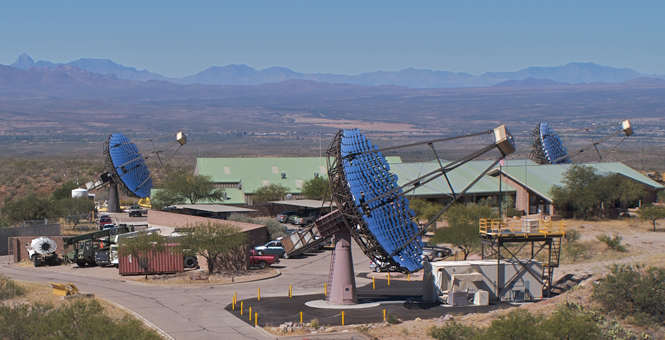
\includegraphics[width=300px]{VERITAS.jpg}
    \end{figure}
\end{frame}


\begin{frame}{ICAT: VERITAS}
    Location: 31 \textdegree43043'' N, 110\textdegree57'07'' W at 1268 m
    \newline
    Detection method:  Cherenkov technique
    \begin{figure}[h]
        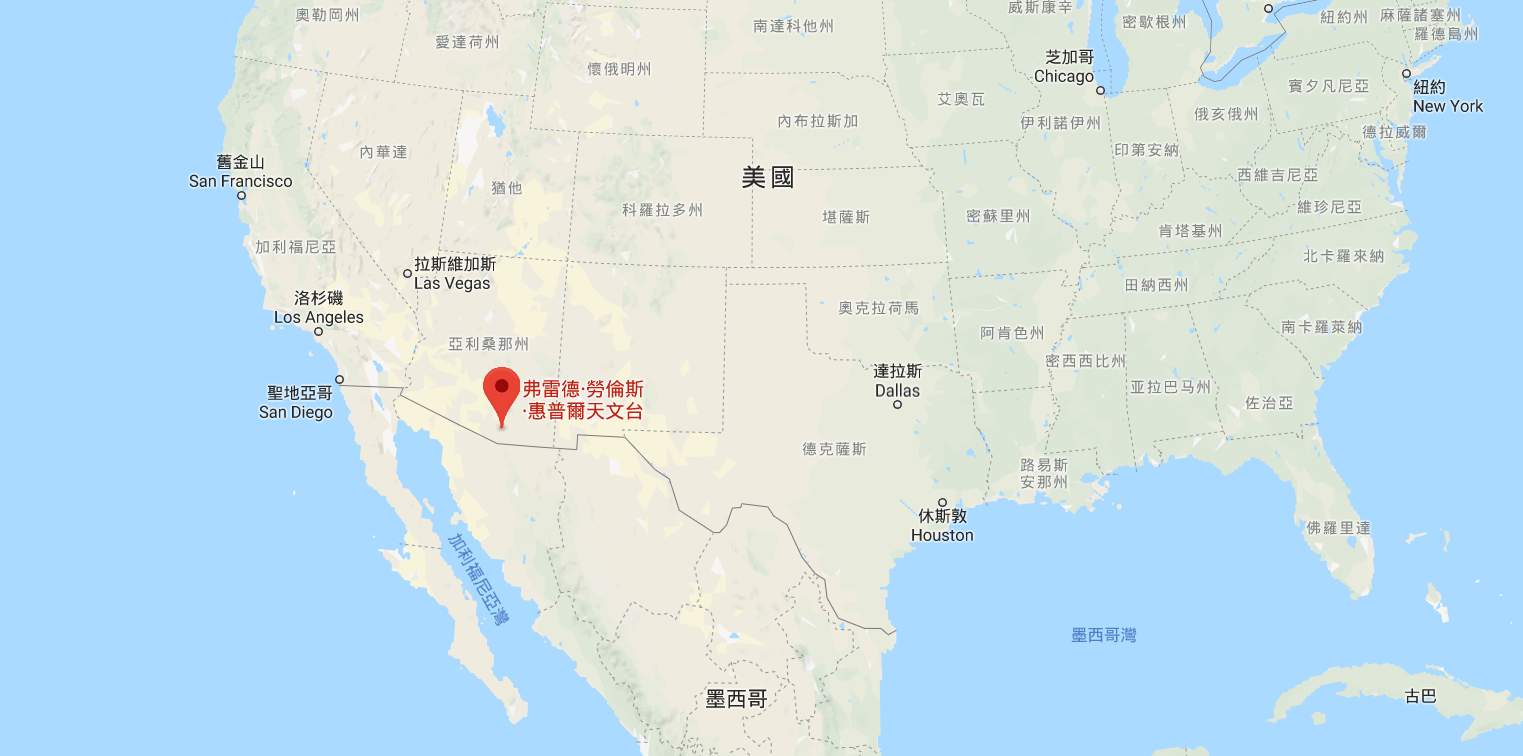
\includegraphics[width=300px]{VERITAS_location.png}
    \end{figure}
\end{frame}


% target source
\begin{frame}{ICAT: VERITAS}
    observed sources
    \begin{itemize}
        \item blazars
        \item black holes at the centres of active galaxies
        \item pulsars
        \item X-ray binaries
        \item gamma-ray bursts
        \item supernova remnants
        \item globular clusters
        \item galaxies including our own Milky Way Galaxy.
        \item Galaxy clusters
    \end{itemize}
\end{frame}


\begin{frame}{ICAT: VERITAS}
    \begin{figure}[h]
        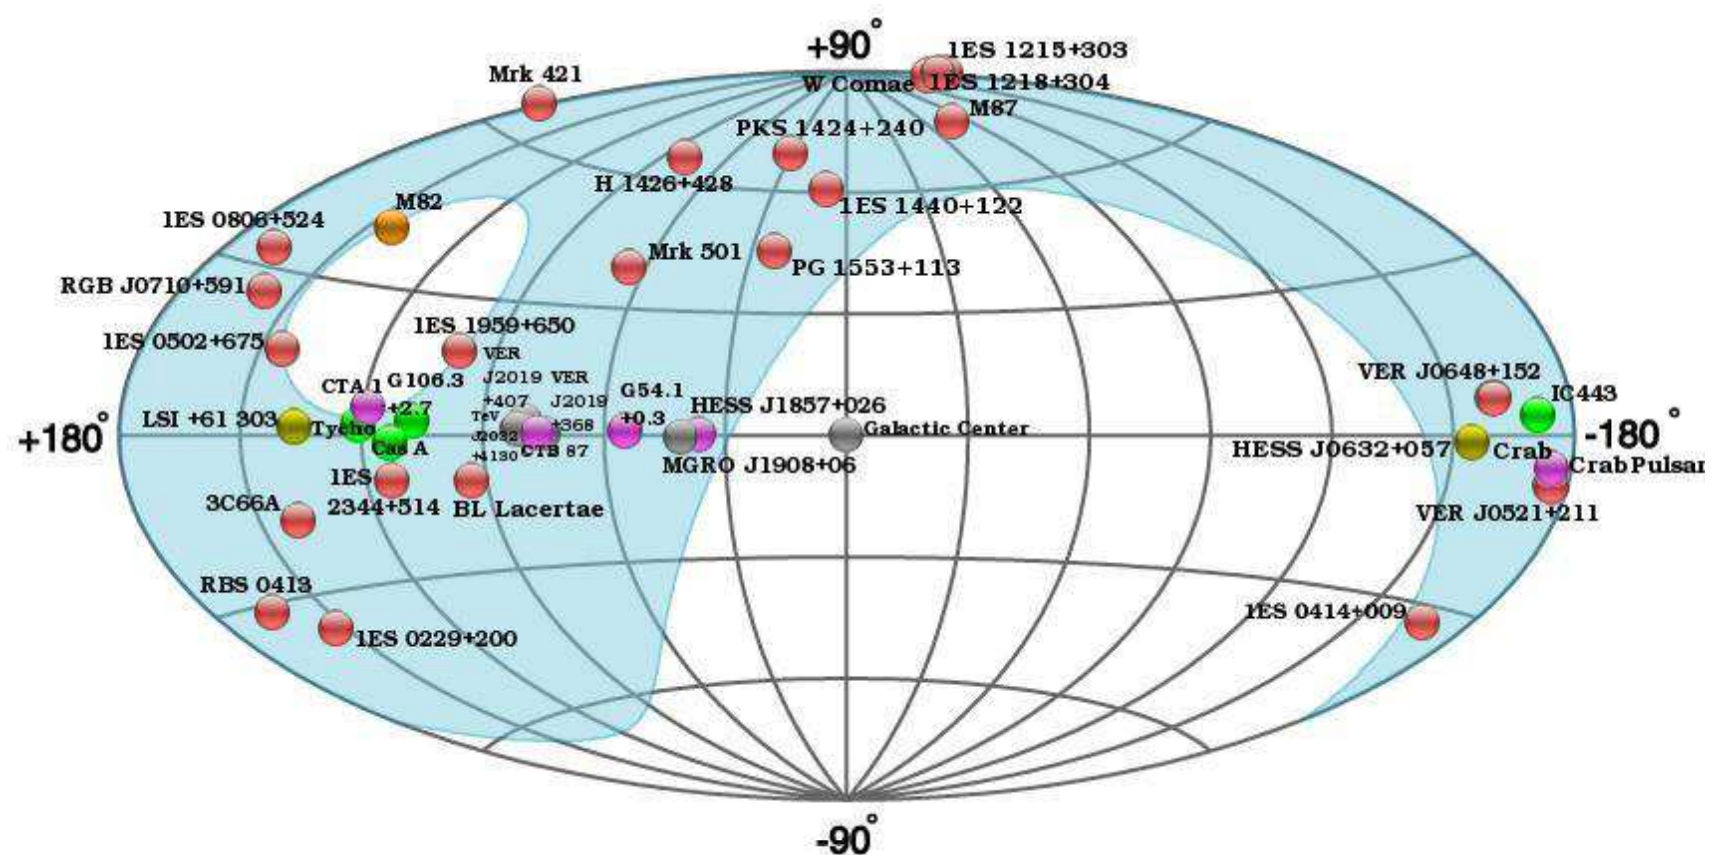
\includegraphics[width=300px]{VERITAS_source_map.png}
        \caption{The VERITAS source map, in Galactic coordinates, as of July 2011}
    \end{figure}
\end{frame}


% collaboration
\begin{frame}{ICAT: VERITAS}
    Fred Lawrence Whipple Observatory
    \begin{itemize}
        \item $\sim$ 80 scientists
        \item $>$ 4 countries
    \end{itemize}
    \begin{figure}[h]
        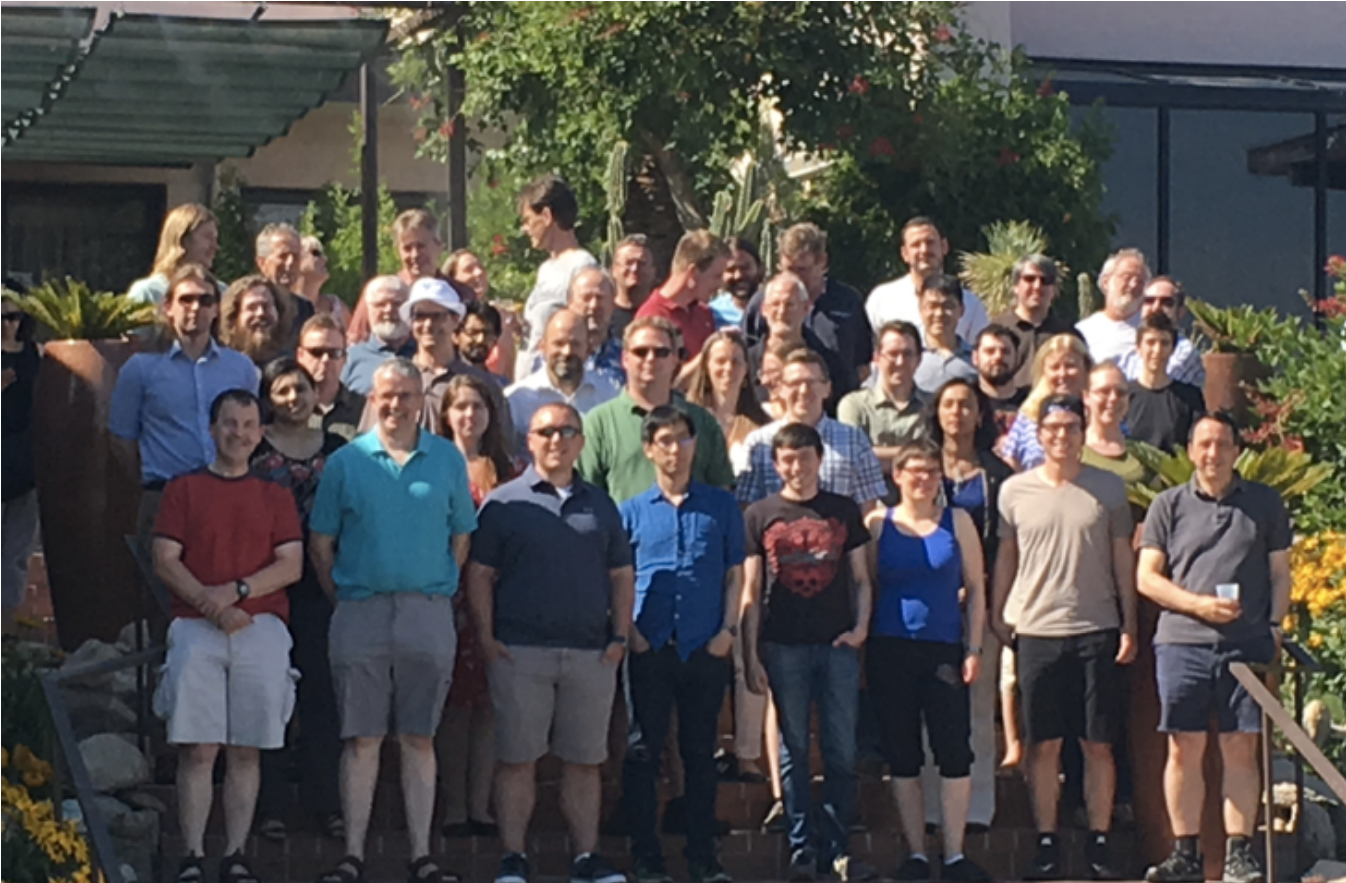
\includegraphics[width=270px]{VERITAS_collaboration.png}
    \end{figure}
\end{frame}


% history
\begin{frame}{ICAT: VERITAS}
    Brief history:
    \begin{enumerate}
        \item April 2003, Installation of VERITAS prototype telescope at the FLWO Basecamp
        \item February 2004, First light of VERITAS prototype
        \item January 2007, Completion of 4 telescope array
        \item April 27-28 2007, First Light Celebration
        \item Summer 2009, Displacement of Telescope 1 to new location for improved sensitivity
        \item Summer 2012, Upgrade of camera PMTs to high-quantum-efficiency PMTs
    \end{enumerate}
\end{frame}


% telescope
\begin{frame}{ICAT: VERITAS}
    VERITAS telescope
    \begin{itemize}
        \item based on Davies–Cotton design
        \item 12 m radius spherical surface
        \item echo reflector carries 315 mirrors
        \item mirror area $\sim$ 100 $ \text{m}^2$
    \end{itemize}
\end{frame}


\begin{frame}{ICAT: VERITAS}
    \begin{figure}[h]
        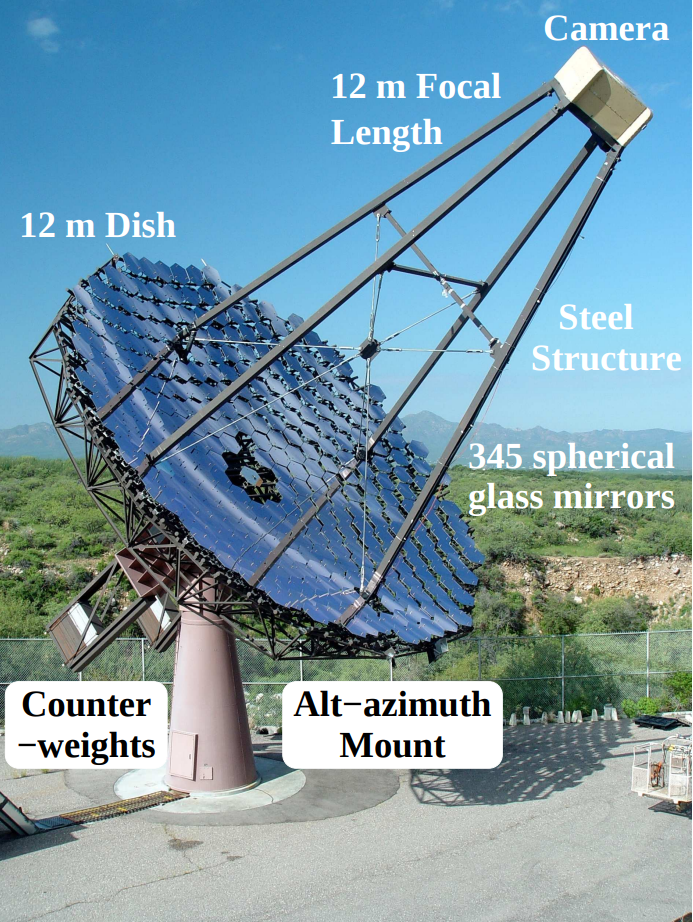
\includegraphics[width=150px]{VERITAS_telescope.png}
    \end{figure}
\end{frame}


\begin{frame}{ICAT: VERITAS}
    blue: original layout
    \newline
    red: new layout
    \begin{figure}[h]
        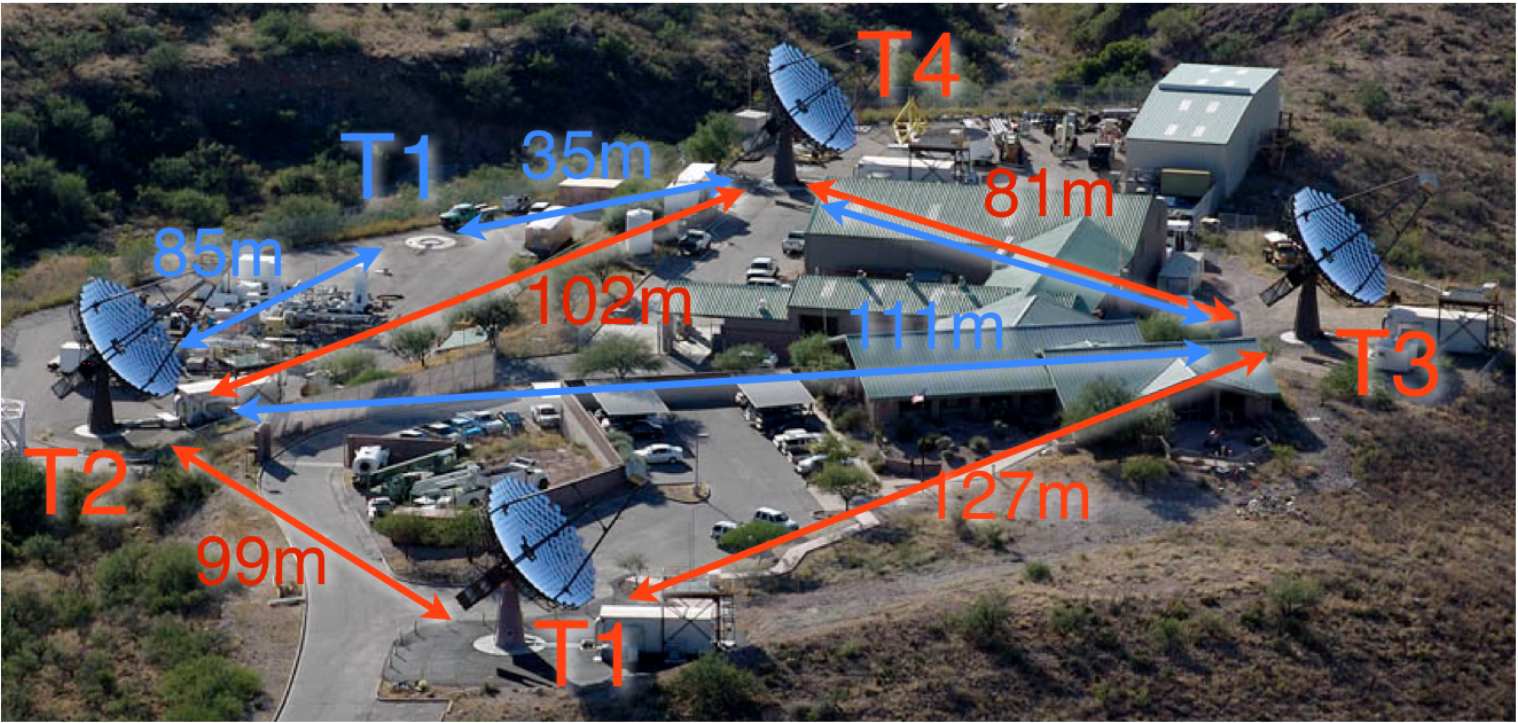
\includegraphics[width=330px]{VERITAS_array.png}
    \end{figure}
\end{frame}


% camera
\begin{frame}{ICAT: VERITAS}
    VERITAS camera
    \begin{itemize}
        \item 499 pixels/camera
        \item Energy range: 50 GeV to 30 TeV
        \item Energy resolution: 20 \% \@ 1 TeV
        \item Angular resolution (68 \% containment): 0.08° \@ 1 TeV
        \item Point source sensitivity: 1 \% Crab in $\sim$ 25h
        \item 28 mm Photonis phototubes
    \end{itemize}
    \begin{figure}[h]
        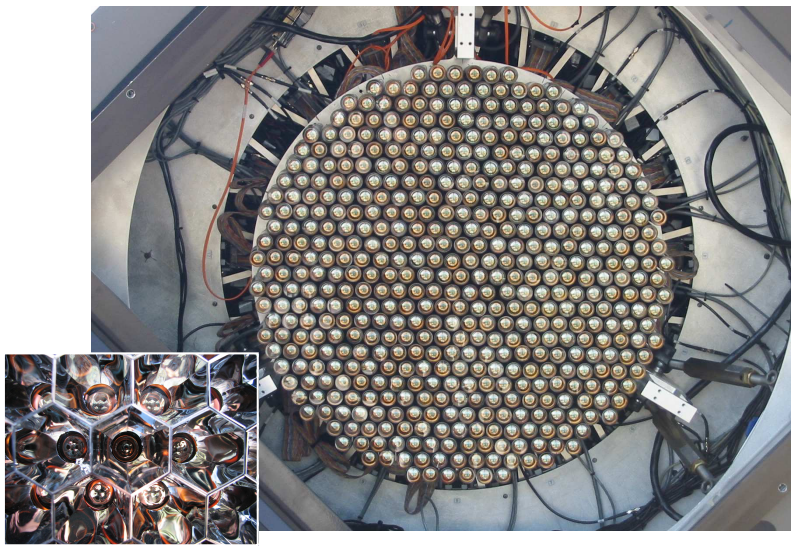
\includegraphics[width=180px]{VERITAS_camera.png}
    \end{figure}
\end{frame}


% mirror
\begin{frame}{ICAT: VERITAS}
    VERITAS mirror
    \begin{itemize}
        \item area is approximately 106 $\text{m}^2$
        \item  24m radius of curvature of each mirror
    \end{itemize}

    \begin{figure}[h]
        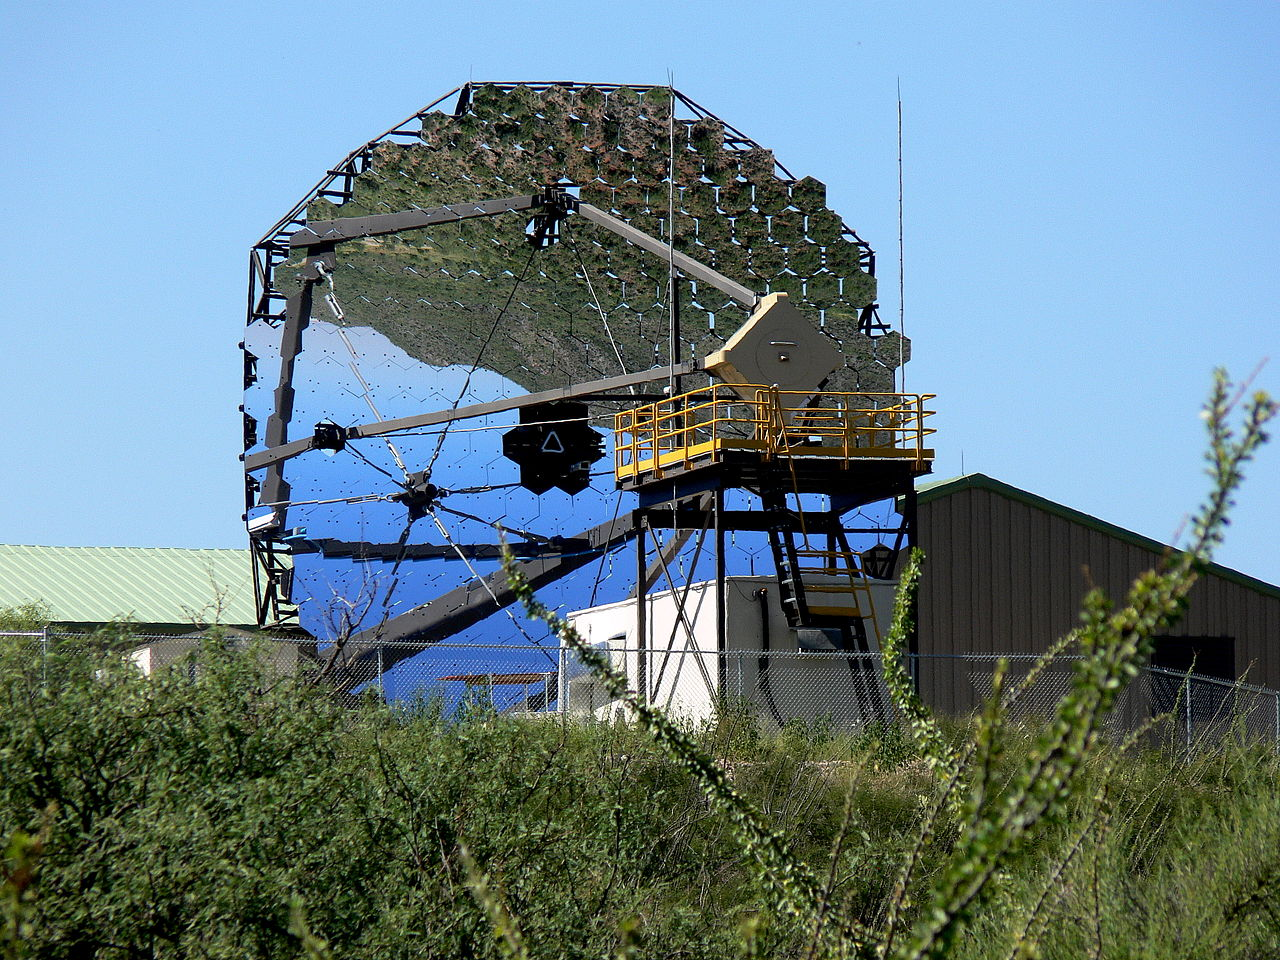
\includegraphics[width=220px]{VERITAS_mirror.jpg}
    \end{figure}
\end{frame}


% upgrade
\begin{frame}{ICAT: VERITAS}
    VERITAS upgrade
    \begin{itemize}
        \item  photomultiplier tubes: more sensitive, superbialkali devices
        \item trigger system: higher speed, FGPA-based device
        \item Upgrading inter-telescope networking and communications
        \item Adding instrumentation to the central pixels $\Rightarrow$ high-speed optical monitoring and stellar intensity interferometry
    \end{itemize}
\end{frame}



\begin{frame}{ICAT: VERITAS}
    \begin{figure}[h]
        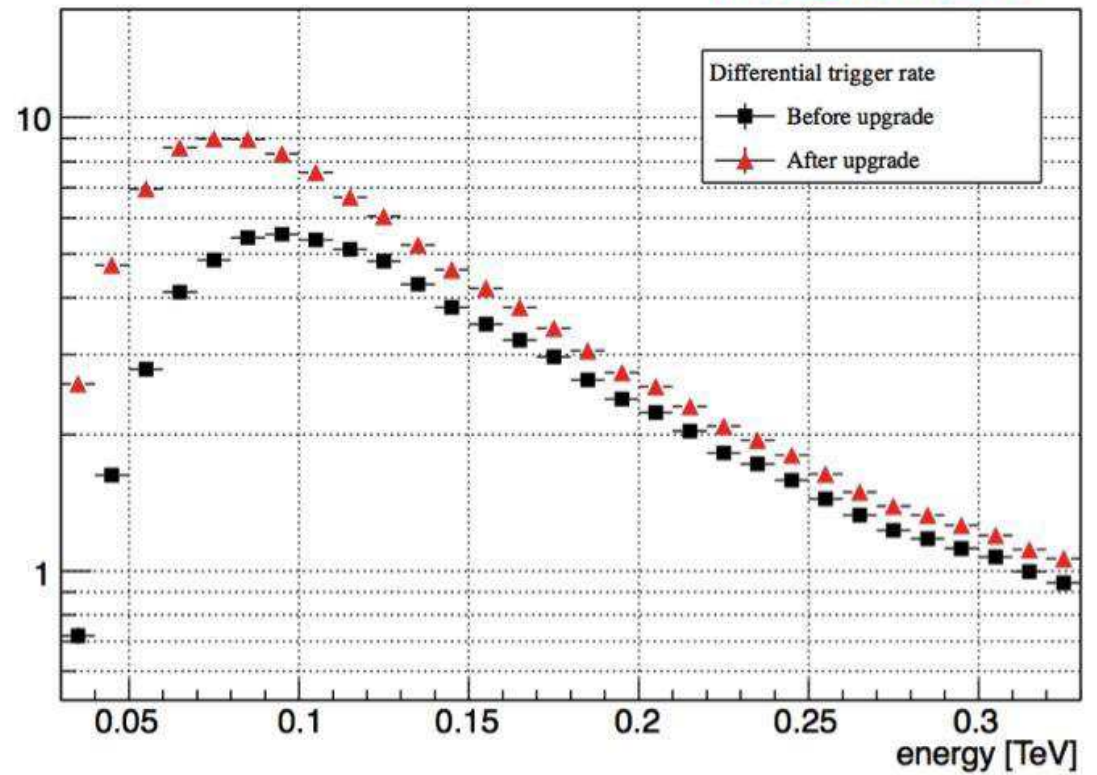
\includegraphics[width=300px]{VERITAS_upgrade.png}
    \end{figure}
\end{frame}


% result
\begin{frame}{ICAT: VERITAS}
\end{frame}


\end{document}